\chapter{Síťová komunikace a databáze} \label{chap:methods}

Smyslem zkonstruovaných čidel je jejich snadná implementace do bytu či domu. \\
ESP8266 potřebuje jen napájení, celá komunikace mezi mikročipem a brokerem probíhá po WiFi \\

\section{Protokol MQTT} \label{sec:protocol_mqtt}

Co je to protokol MQTT (vznik, využití) \\
Proč zrovna tento protokol \\
Princip použití protokolu MQTT (v síti je broker, který čeká na příchozí zprávy, ostatní zařízení jsou v módu publish - odesílají zprávy na broker, hierarchie zpráv, ...) \\
Zprovoznění komunikace přes MQTT \\ 
Sestavení struktury zpráv + identifikátorů čidel (popis jednotlivých atributů ve zprávě, proč jedno esp může posílat více zpráv do různých topiců, popis zvolené hierarchie topiců, ...) \\
ESP má aktuální čas pomocí NTP protokolu - díky tomu je možné přidávat do zpráv timestampy
Popis logiky odesílání zpráv z ESP - ESP odešle zprávu periodicky vždy v polovině minuty (např.: 14:30:30, 14:31:30, ... ) - lehké nepřesnosti způsobené dobou načítání dat ze senzorů, ... \\

%\begin{figure}[H]
  %\centering
  %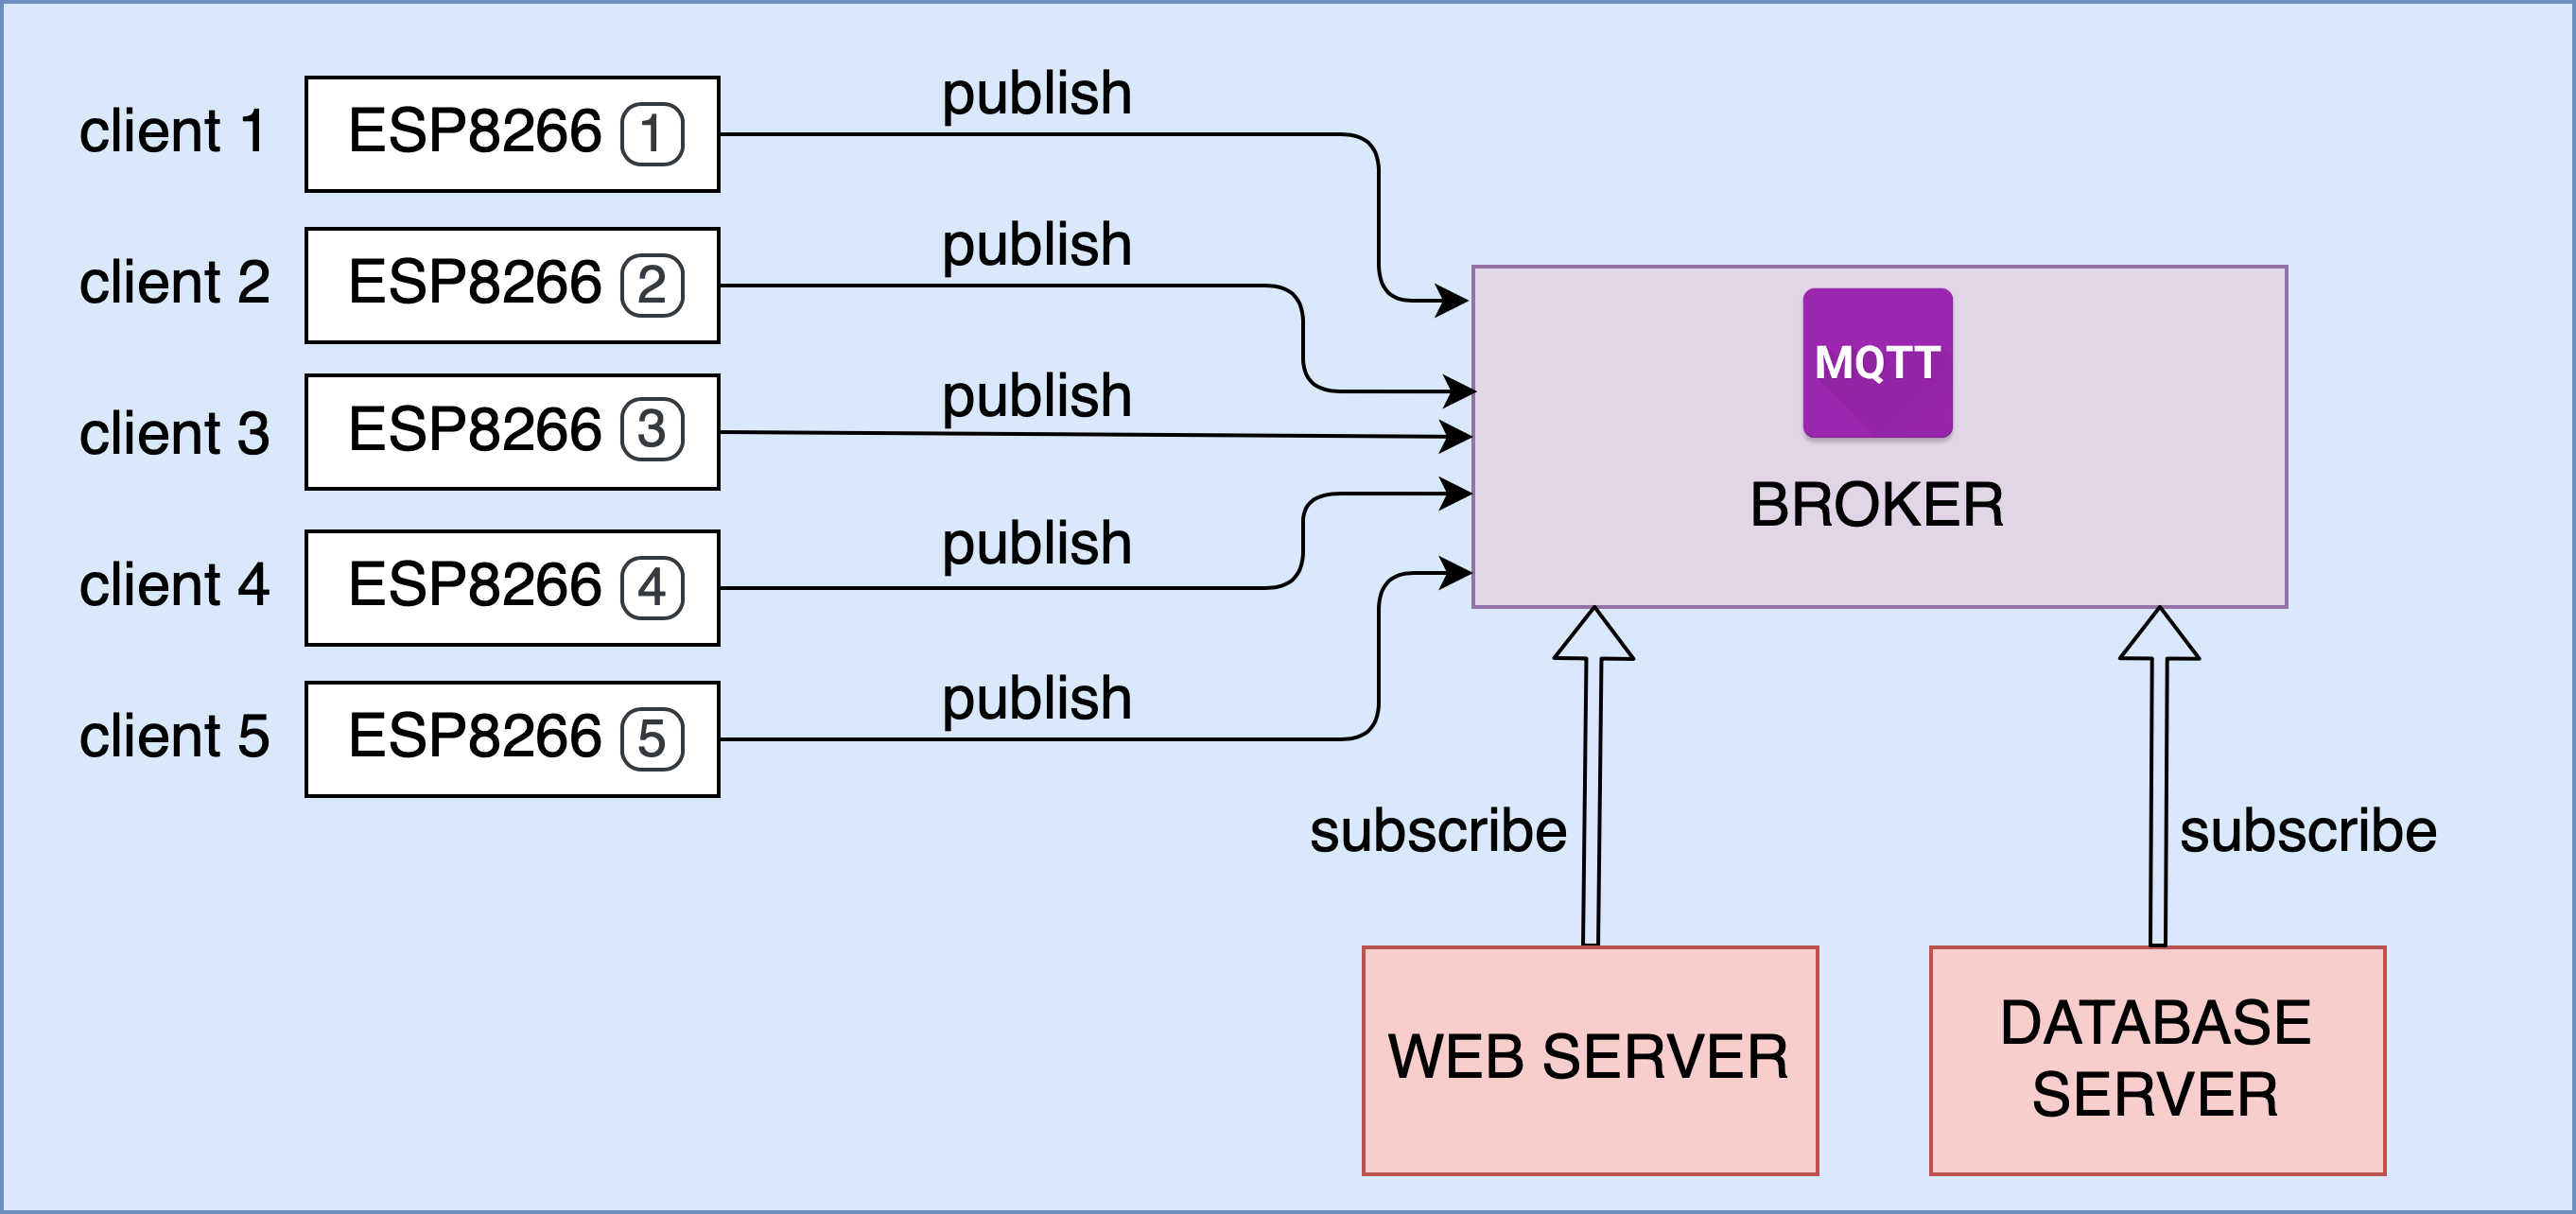
\includegraphics[width=0.7 \textwidth]{mqtt_diagram.png}
  %\caption{POPIS}
  %\label{fig:schema_esp_bme280}
%\end{figure}

\section{Ukládání dat do databáze} \label{sec:database}

Základní princip databáze, proč jsme se rozhodli pro použití databáze,  ... \\
Co je MongoDB (určení, využití, funkčnost, ... ) \\
Ukládání hodnot měřených veličin do MongoDB \\

\section{Webserver} \label{sec:webserver}

Popis backendu engine.py
Backend - z hlediska programování - jeden soubor engine.py, který zajišťuje serverování webové stránky, ukládání dat do databáze, sensor check, ... \\